\section{MODHYDROLOG (model ID: 36)}
The MODHYDROLOG model (fig.~\ref{fig:36_schematic}) is an elaborate groundwater recharge model, originally created for use in Australia \citep{Chiew1990,Chiew1994}. It has 5 stores (I, D, SMS, GW and CH) and 15 parameters (INSC, COEFF, SQ, SMSC, SUB, CRAK, EM, DSC, ADS, MD, VCOND, DLEV, $k_1$, $k_2$ and $k_3$). It originally includes a routing scheme that allows linking sub-basins together, which has been removed here. The model aims to represent:

\begin{itemizecompact}
\item Interception by vegetation;
\item Infiltration and infiltration excess flow;
\item Depression storage and delayed infiltration;
\item Preferential groundwater recharge, interflow and saturation excess flow;
\item Groundwater recharge resulting from filling up of soil moisture storage capacity;
\item Water exchange between shallow and deep aquifers;
\item Water exchange between aquifer and river channel.
\end{itemizecompact}

\subsection{MARRMoT model name}
m\_36\_modhydrolog\_15p\_5s \\

% Equations
\subsection{Model equations}

% Model layout figure
{ 																	% This ensures it doesn't warp text further down
\begin{wrapfigure}{l}{7cm}
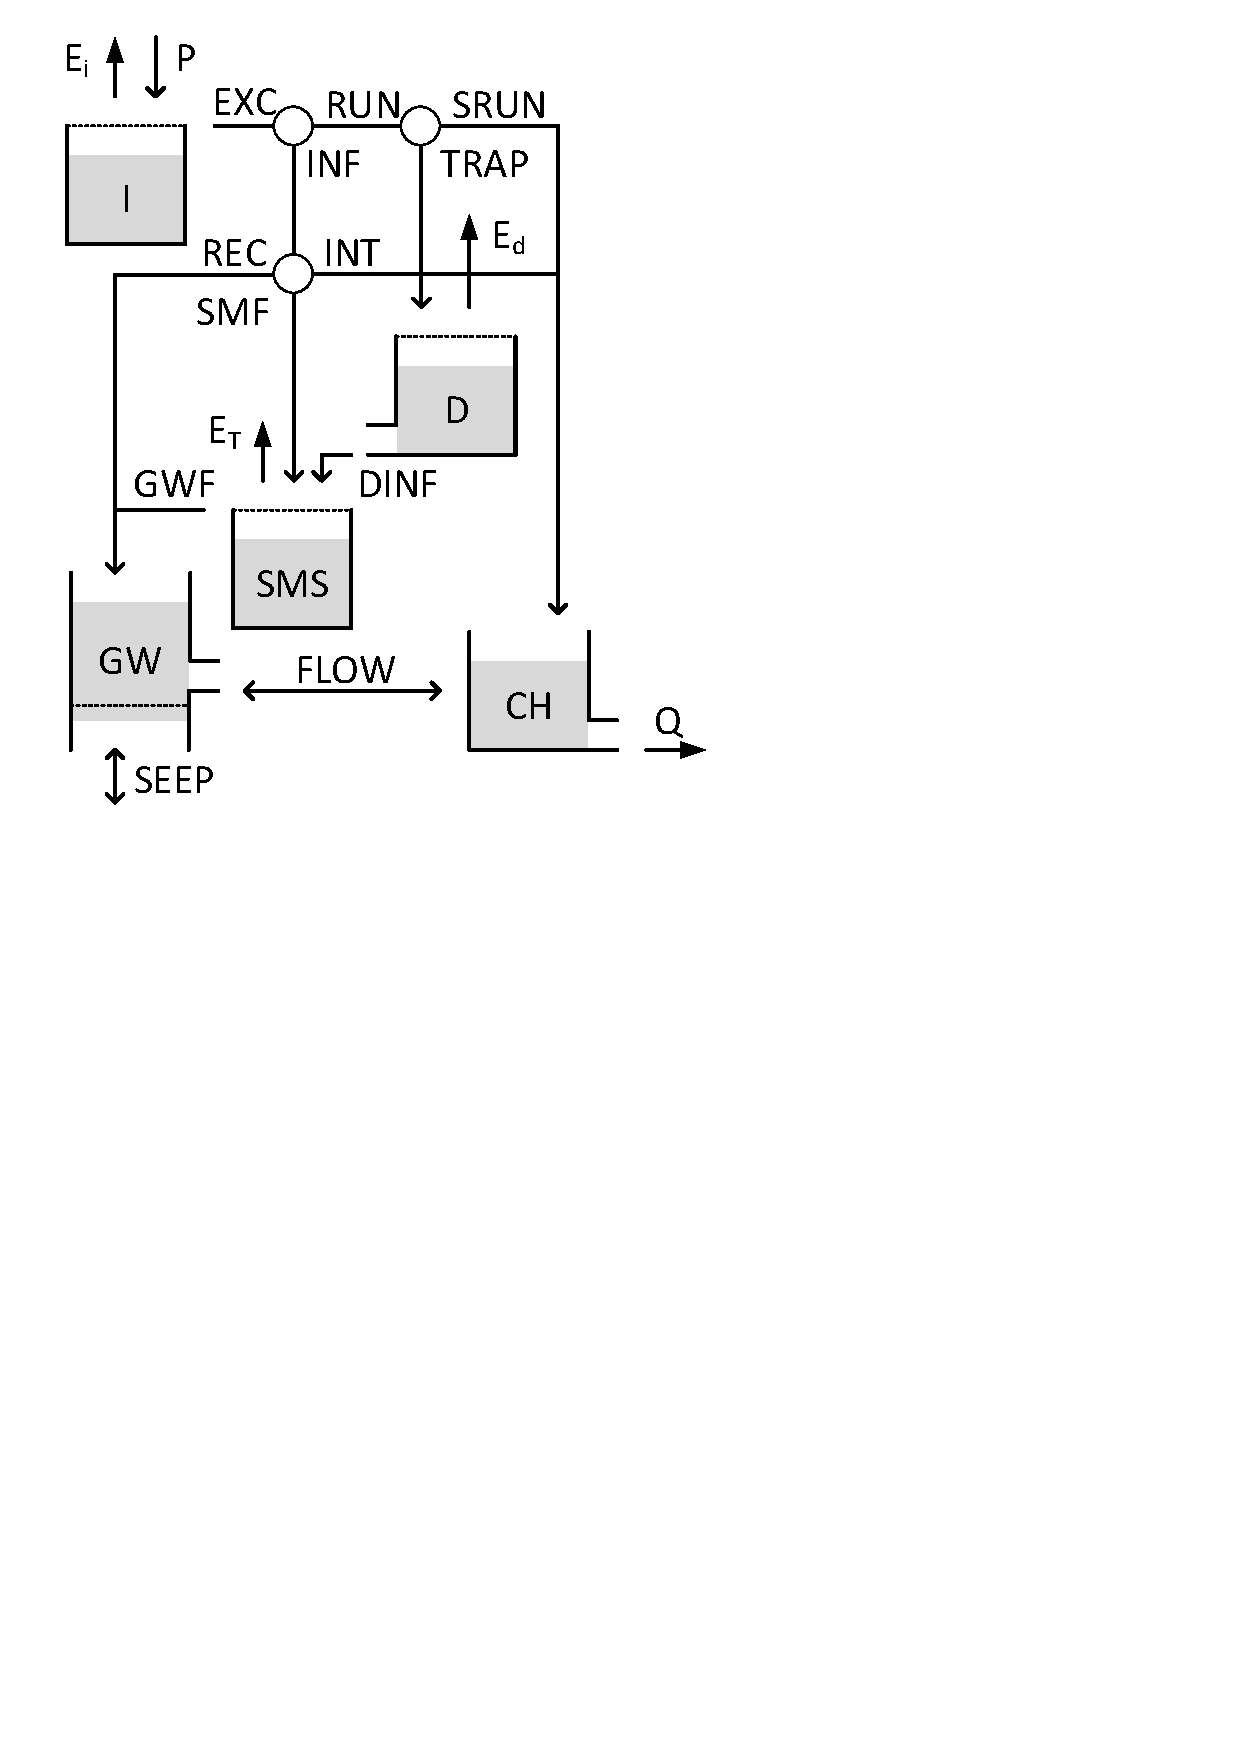
\includegraphics[trim=1cm 16.5cm 9cm 1cm,width=7cm,keepaspectratio]{./AppA_files/36_schematic.pdf}
\caption{Structure of the MODHYDROLOG model} \label{fig:36_schematic}
\end{wrapfigure}

\begin{align}
	\frac{dI}{dt} &= P-E_i-EXC \\
	E_i &= \begin{cases}
		E_p, &\text{if } I > 0 \\
		0, & \text{otherwise} \\
	\end{cases} \\
	EXC &= 
	\begin{cases}
		P, & \text{if } I = INSC \\
		0, & \text{otherwise}
	\end{cases}
\end{align}

Where I [mm] is the current interception storage, $P$ the rainfall [mm/d], $E_i$ the evaporation from the interception store [mm/d] and $EXC$ the excess rainfall [mm/d]). Evaporation is assumed to occur at the potential rate $E_p$ [mm/d] when possible. When I exceeds the maximum interception capacity $INSC$ [mm], water is routed to the rest of the model as excess precipitation $EXC$. The soil moisture store SMS is instrumental in dividing runoff between infiltration and surface flow:

} % end of wrapfigure fix

\vspace{1cm}
\begin{align}
	\frac{dSMS}{dt} &= SMF+DINF-E_T-GWF\\
	SMF &= INF-INT-REC\\
		&INF = min\left(COEFF * exp\left(\frac{-SQ*SMS}{SMSC}\right),EXC\right)\\
		&INT = SUB*\frac{SMS}{SMSC} * INF \\
		&REC = CRAK*\frac{SMS}{SMSC}*(INF-INT)\\	
	E_T &=min\left(EM*\frac{SMS}{SMSC},PET\right)\\
	GWF &= \begin{cases}
		SMF, &\text{if } SMS = SMSC\\
		0, &\text{otherwise}
	\end{cases}
\end{align}

Where SMS is the current storage in the soil moisture store [mm]. SMF [mm/d] and DINF [mm/d] are the infiltration and delayed infiltration respectively. INF is total infiltration [mm/d] from excess precipitation, based on maximum infiltration loss parameter COEFF [-], the infiltration loss exponent SQ [-] and the ratio between current soil moisture storage SMS [mm] and the maximum soil moisture capacity SMSC [mm]. INT represents interflow and saturation excess flow [mm/d], using a constant of proportionality SUB [-]. REC is preferential recharge of groundwater [mm/d] based on another constant of proportionality CRAK [-]. SMF is flow into soil moisture storage [mm/d]. $E_T$ evaporation from the soil moisture that occurs at the potential rate when possible [mm/d], based on the maximum plant-controlled rate EM [mm/d]. GWF is the flow to the groundwater store [mm/d]:

\begin{align}
	\frac{dD}{dt} &= TRAP - E_D - DINF \\
	TRAP &= ADS*exp\left(-MD\frac{D}{DSC-D}\right)*RUN\\
		&RUN = EXC-INF\\
	E_D &= \begin{cases}
			ADS*E_p, &\text{if } D > 0 \\
			0, &\text{otherwise} \\
		\end{cases}\\
	DINF &= \begin{cases}
			ADS*RATE, &\text{if }  D > 0\\
			0, &\text{otherwise} \\
		\end{cases} \\
		&RATE = COEFF*exp\left(-SQ\frac{SMS}{SMSC}\right) - INF-INT-REC
\end{align}

Where TRAP [mm/d] is the part of overland flow captured in the depression store (equation taken from \citet{Porter1971}), $E_D$ the evaporation from the depression store [mm/d], and DINF delayed infiltration to soil moisture [mm/d]. TRAP uses DSC as the maximum depression store capacity [mm], ADS as the fraction of land functioning as depression storage [-] and MD a depression storage parameter [-]. $E_D$ relies on the potential evapotranspiration $E_p$. The groundwater store has no defined upper and lower boundary and instead fluctuates around a datum DLEV [mm]:

\begin{align}
	\frac{dGW}{dt} &= REC+GWF - SEEP - FLOW\\
	SEEP &= VCOND*\left(GW - DLEV\right) \\
	FLOW &= \begin{cases}
			k_1*|GW|+k_2*\left(1-exp(-k_3*|GW|)\right), &\text{if } GW \geq 0\\
			-\left(k_1*|GW|+k_2*\left(1-exp(-k_3*|GW|)\right)\right), &\text{if } GW < 0\\
		\end{cases}
\end{align}

Where SEEP [mm/d] is the exchange with a deeper aquifer (can be negative or positive) and FLOW [mm/d] the exchange with the channel (can be negative or positive). VCOND $[d^{-1}]$ is a leakage coefficient, DLEV a datum around which the groundwater level can fluctuate, and $k_1$, $k_2$ and $k_3$ are runoff coefficients. The channel store aggregates incoming fluxes and produces the total runoff $Q_t$ [mm/d]:

\begin{align}
	\frac{dCH}{dt} &= SRUN + INT + FLOW - Q \\
	SRUN &= RUN-TRAP \\
	Q_t &= \begin{cases}
		CH, &\text{if } CH > 0\\
		0, &\text{otherwise}
	\end{cases}
\end{align}

\newpage
\subsection{Parameter overview}
% Table generated by Excel2LaTeX from sheet 'Sheet1'
\begin{table}[htbp]
  \centering
    \begin{tabular}{lll}
    \toprule
    Parameter & Unit  & Description \\
    \midrule
    INSC  & $mm$  & Maximum interception capacity \\
    COEFF & $mm~d^{-1}$ & Maximum infiltration loss \\
    SQ    & $-$   & Infiltration loss exponent \\
    SMSC  & $mm$  & Maximum soil moisture storage \\
    SUB   & $-$   & Proportionality constant \\
    CRAK  & $-$   & Proportionality constant \\
    EM    & $mm~d^{-1}$ & Maximum plant-controlled evaporation rate \\
    DSC   & $mm$  & Maximum depression storage \\
    ADS   & $-$   & Fraction of area functioning as depression store \\
    MD    & $-$   & Depression store shape parameter \\
    VCOND & $d^{-1}$ & Runoff coefficient \\
    DLEV  & $mm$  & Datum of groundwater store \\
    $k_1$ & $d^{-1}$ & Runoff coefficient \\
    $k_2$ & $d^{-1}$ & Runoff coefficient \\
    $k_3$ & $d^{-1}$ & Runoff coefficient \\
    \bottomrule
    \end{tabular}%
  \label{tab:addlabel}%
\end{table}%
